\documentclass[10pt]{beamer}
\usepackage{SexySlides1,fancyvrb,outlines,pbox}
\usepackage[round]{natbib}
\usepackage{hyperref} % link references
\hypersetup{colorlinks = true, citecolor = red, urlcolor = blue}
\usepackage[font=footnotesize]{caption} % caption options
\usepackage{fancyvrb}

\theoremstyle{definition}
\newtheorem{Algorithm}{Algorithm}


\usepackage[tikz]{bclogo}
\presetkeys{bclogo}{
ombre=true,
epBord=3,
couleur = white,
couleurBord = black,
arrondi = 0.2,
logo=\bctrombone
}{}

\definecolor{UniBlue}{RGB}{83,121,170}
\setbeamercolor{title}{fg=UniBlue}
\setbeamercolor{frametitle}{fg=UniBlue}
\newcommand{\coluit}{\color{UniBlue}\it}
\newcommand{\colubf}{\color{UniBlue}\bf}
\DeclareMathOperator*{\diag}{diag}
\DeclareMathOperator*{\Tr}{Tr}
\DeclareMathOperator*{\argmin}{argmin}
\DeclareMathOperator*{\ve}{vec}
\DeclareMathOperator*{\Th}{\text{th}}
\DeclareMathOperator*{\supp}{\text{supp}}

% Row color change in table
\makeatletter
\def\zapcolorreset{\let\reset@color\relax\ignorespaces}
\def\colorrows#1{\noalign{\aftergroup\zapcolorreset#1}\ignorespaces}
\makeatother

     \setbeamertemplate{footline}
        {
      \leavevmode%
      \hbox{%
      \begin{beamercolorbox}[wd=.333333\paperwidth,ht=2.25ex,dp=1ex,center]{author in head/foot}%
        \usebeamerfont{author in head/foot}\insertshortauthor~~
        %(\insertshortinstitute)
      \end{beamercolorbox}%
      \begin{beamercolorbox}[wd=.333333\paperwidth,ht=2.25ex,dp=1ex,center]{title in head/foot}%
        \usebeamerfont{title in head/foot}\insertshorttitle
      \end{beamercolorbox}%
      \begin{beamercolorbox}[wd=.333333\paperwidth,ht=2.25ex,dp=1ex,right]{date in head/foot}%
        \usebeamerfont{date in head/foot}\insertshortdate{}\hspace*{2em}

    %#turning the next line into a comment, erases the frame numbers
        %\insertframenumber{} / \inserttotalframenumber\hspace*{2ex} 

      \end{beamercolorbox}}}%

%\def\logo{%
%{\includegraphics[height=1cm]{goldy1.png}}
%}
%%
%\setbeamertemplate{footline}
%{%
%	\hspace*{.05cm}\logo
%  \begin{beamercolorbox}[sep=1em,wd=10cm,rightskip=0.5cm]
%  {footlinecolor,author in head/foot}
%%    \usebeamercolor{UniBlue}
%    \vspace{0.1cm}
%    \insertshortdate \hfill \insertshorttitle
%    \newline
%    \insertshortauthor   - \insertshortinstitute
%    \hfill
%    \hfill \insertframenumber/\inserttotalframenumber
%  \end{beamercolorbox}
%  \vspace*{0.05cm}
%}

%% smart verbatim
\fvset{framesep=1cm,fontfamily=courier,fontsize=\scriptsize,framerule=.3mm,numbersep=1mm,commandchars=\\\{\}}

\title[Joint Multi${}^2$ GGM]
{\Large  
Joint Estimation and Inference for Multiple Multi-layered Gaussian Graphical Models}

\author[Majumdar and Michailidis]{Subhabrata Majumdar and George Michailidis}
\institute[]{University of Florida Informatics Institute\\
\vspace{1em}
IISA-2017 Conference, Hyderabad, India\\
December 28, 2017} 

%\vspace{.5cm}
%\includegraphics[height=.5cm]{UMNlogo}}

%\date [December 28, 2017]

%%%%%%%List Outline in the beginning of each section.
\AtBeginSection[] {
   \begin{frame}
       \frametitle{Outline}
       \tableofcontents[currentsection]
   \end{frame}
}

%-------------------------------------------------------------------
\begin{document}

%\begin{frame}
%%%%%%%%%%%%%%%%%%%%%%%%%%%%%%%%%%%%%%%%%%%%%%%%%%%%%%%%%%%%%%%

\frame{ \titlepage}

%%%%%%%%%%%%%%%%%%%%%%%%%%%%%%%%%%%%%%%%%%%%%%%%%%%%%%%%%%%%%%%

\begin{frame}
\frametitle{Summary}
\begin{itemize}
\item Biological processes in the body have a natural hierarchical structure, e.g. {\colubf Gene > Protein > Metabolite};
\vspace{1em}

\item There are within layer and between-layer connections in this structure.
\end{itemize}

\begin{figure}
\centering
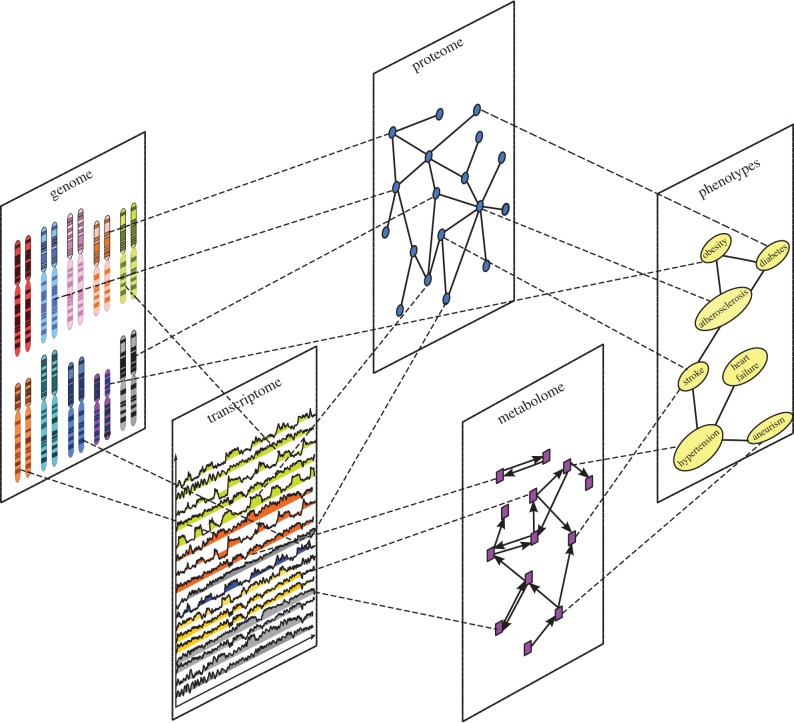
\includegraphics[height=.6\textheight]{data_integration_schematic}
\end{figure}

{\center
{\scriptsize Source: {\colr \cite{GligPrzulj15}}}
}
\end{frame}

%%%%%%%%%%%%%%%%%%%%%%%%%%%%%%%%%%%%%%%%%%%%%%%%%%%%%%%%%%%%%%%
\begin{frame}
\frametitle{Summary}

These connections can be different inside different organs, experimental conditions, or for different subtypes of the same disease;

\begin{center}
\begin{scriptsize}
\begin{tabular}{ccc}
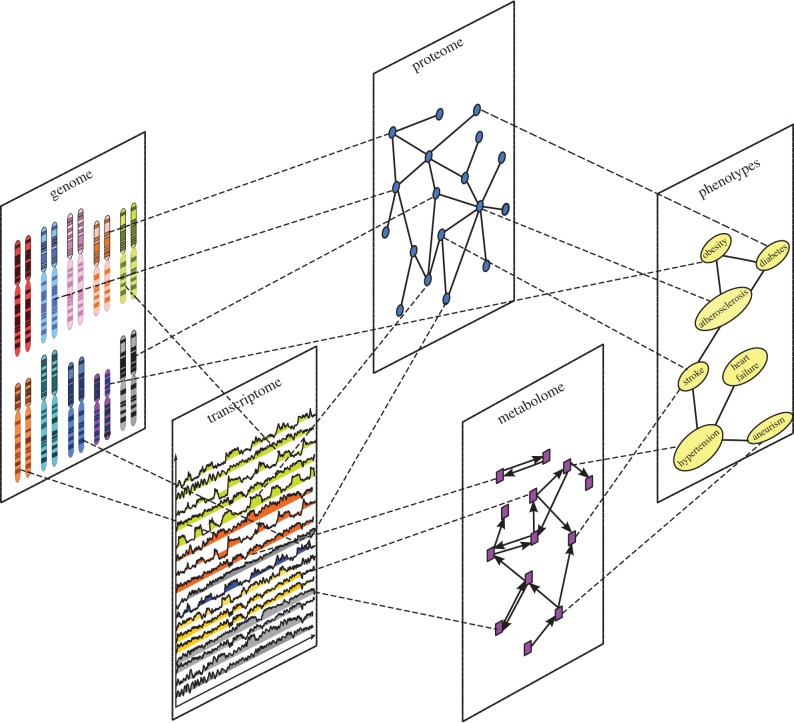
\includegraphics[width=.3\textwidth,angle=-90]{data_integration_schematic}\vspace{.5em}
& 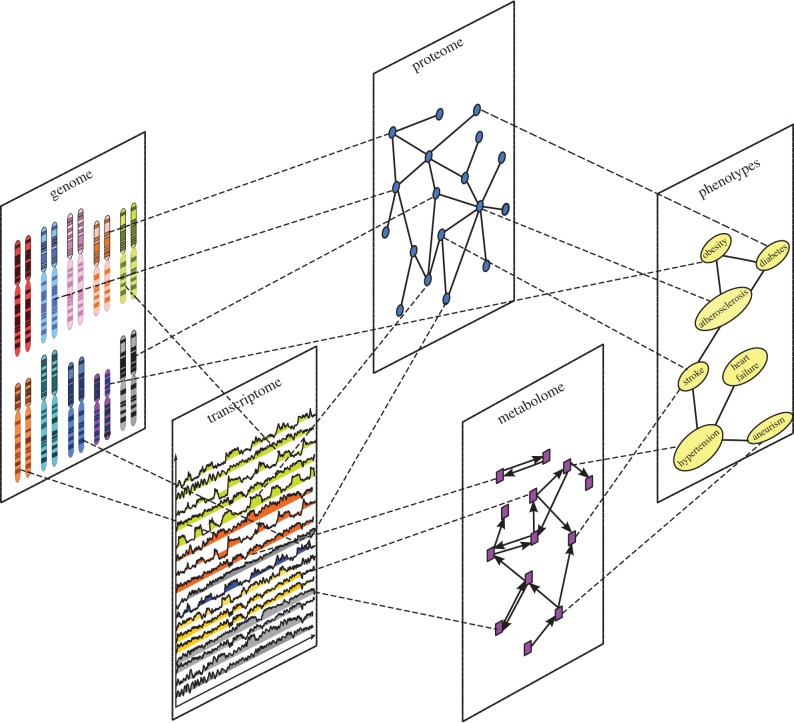
\includegraphics[width=.3\textwidth,angle=-90]{data_integration_schematic}\vspace{.5em}
& 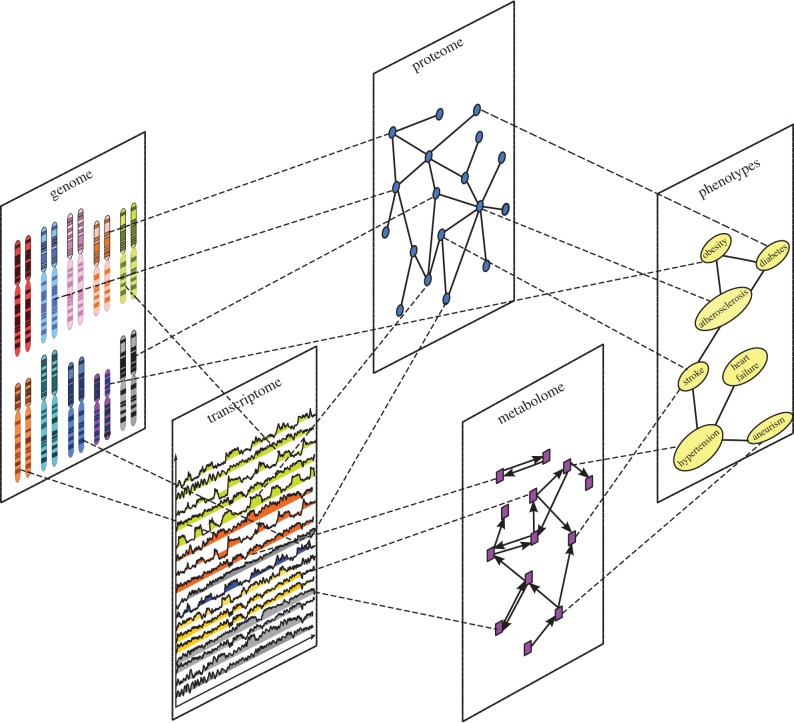
\includegraphics[width=.3\textwidth,angle=-90]{data_integration_schematic}\vspace{.5em}\\
Liver & Kidney & Lungs\\
\end{tabular}
\end{scriptsize}
\end{center}
\end{frame}
%%%%%%%%%%%%%%%%%%%%%%%%%%%%%%%%%%%%%%%%%%%%%%%%%%%%%%%%%%%%%%%

\begin{frame}
\frametitle{What we do}
In this work we propose a general statistical framework based on graphical models for horizontal (i.e. across conditions or subtypes) and vertical (i.e. across different layers containing data on molecular compartments) integration of information in data from such complex biological structures.

\vspace{1em}
Specifically, we perform {\colbit joint estimation and hypothesis testing} for all the connections in these structures.

\end{frame}

%%%%%%%%%%%%%%%%%%%%%%%%%%%%%%%%%%%%%%%%%%%%%%%%%%%%%%%%%%%%%%%%
\section{Formulation of multiple multi-level graphical models}
%%%%%%%%%%%%%%%%%%%%%%%%%%%%%%%%%%%%%%%%%%%%%%%%%%%%%%%%%%%%%%%%

\begin{frame}
\frametitle{Gaussian Graphical models}

\[
\BX = (X_1, \ldots, X_p)^T \sim \cN_p (0, \Sigma_x); \quad
\Omega_x = \Sigma_x^{-1}
\]

\begin{figure}
\centering
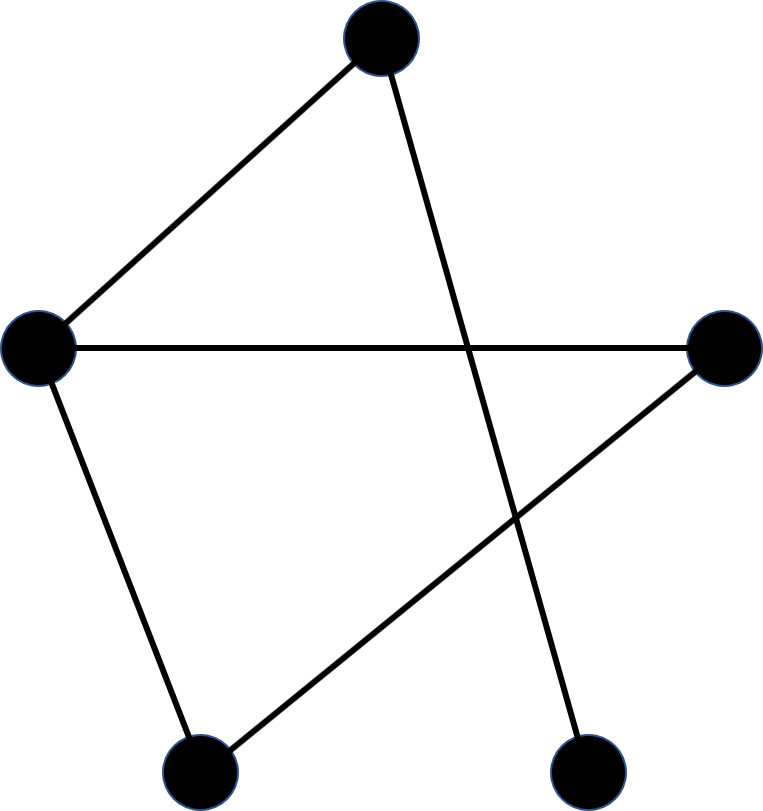
\includegraphics[width=.4\textwidth]{formulation_2}
\end{figure}

Sparse estimation of $\Omega_x$: {\colr \cite{MeisenBuhlmann06}}

Multiple testing and error control: {\colr \cite{DrtonPerlman07}}.

\end{frame}
%%%%%%%%%%%%%%%%%%%%%%%%%%%%%%%%%%%%%%%%%%%%%%%%%%%%%%%%%%%%%%%%

\begin{frame}
\frametitle{Multiple Gaussian Graphical models}

\begin{align*}
& \BX^k = (X_1^k, \ldots, X_p^k)^T \sim \cN_p (0, \Sigma_x^k); \quad
\Omega_x^k = (\Sigma_x^k)^{-1}\\
& k = 1, 2, \ldots, K
\end{align*}

\begin{figure}
\centering
\begin{tabular}{ccc}
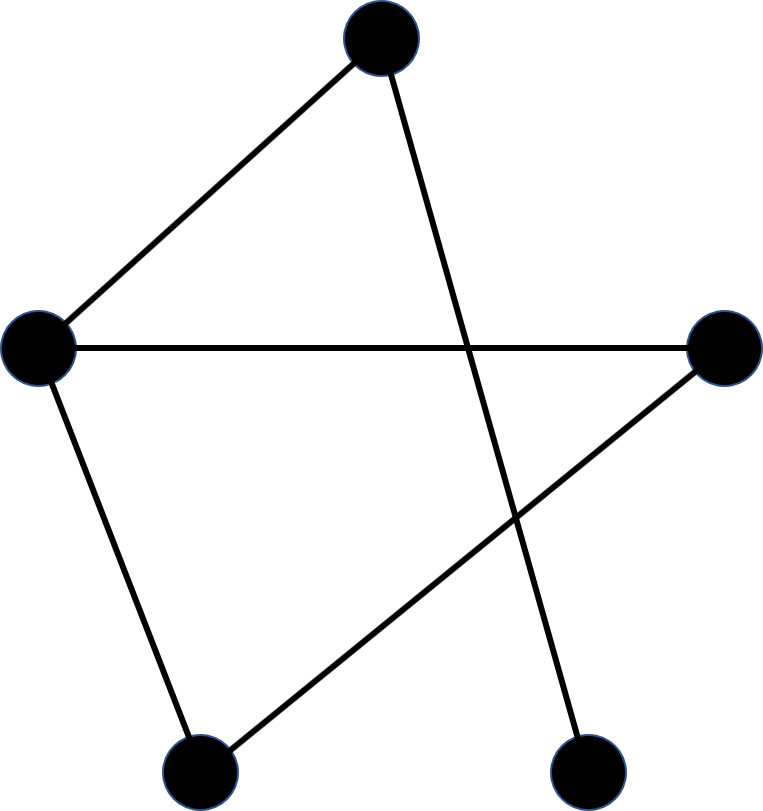
\includegraphics[width=.25\textwidth]{formulation_2} & 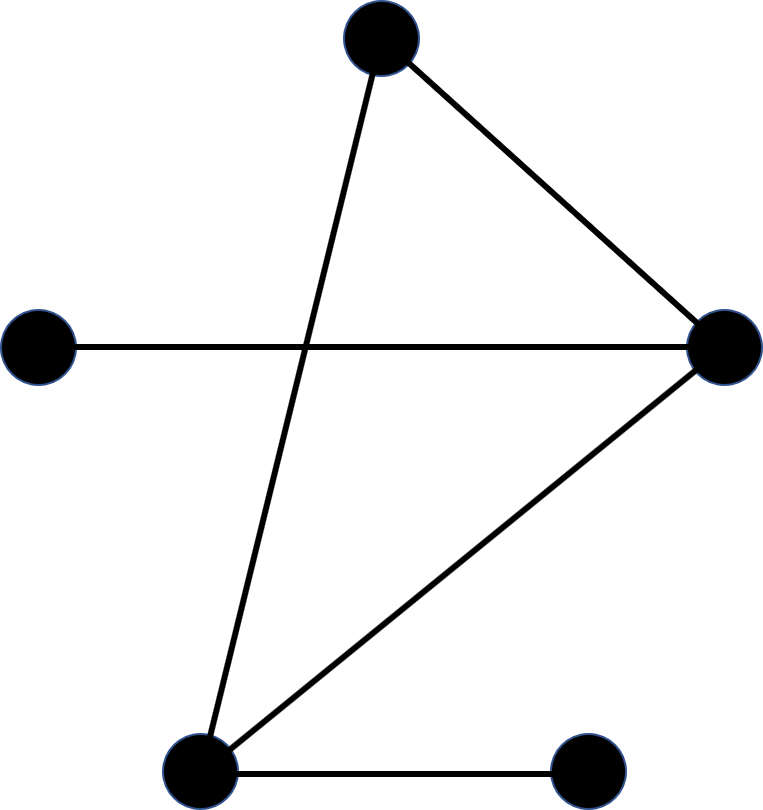
\includegraphics[width=.25\textwidth]{formulation_3}
& 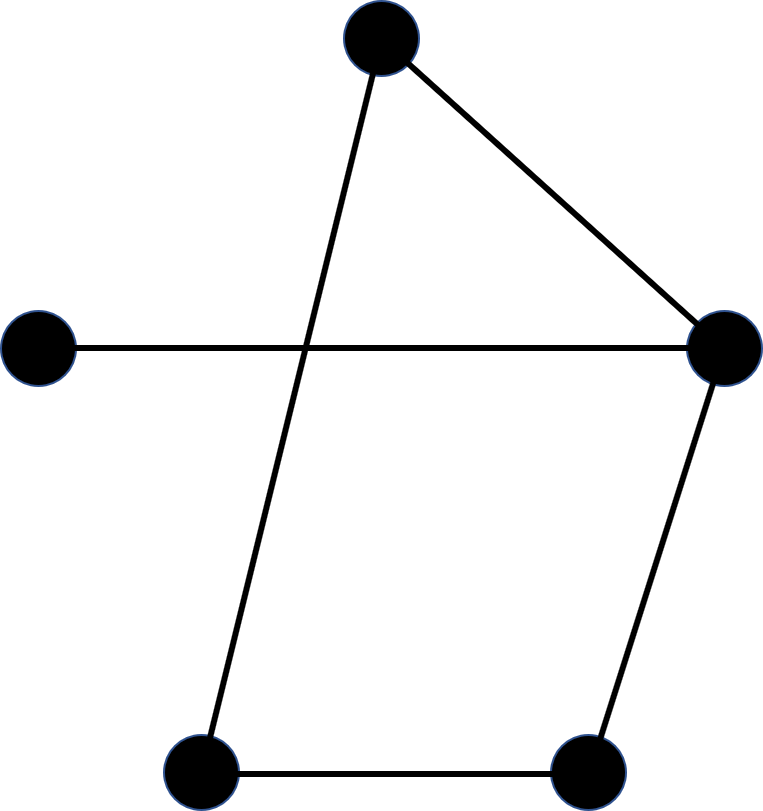
\includegraphics[width=.25\textwidth]{formulation_4}
\\
$k=1$ & $k=2$ & $k=3$
\end{tabular}
\hspace{1em}
\end{figure}
\vspace{1em}

\begin{itemize}
\item Joint estimation of $\{ \Omega_x^k \}$: {\colr \cite{GuoEtal11, MaMichailidis15}}
\vspace{1em}

\item Difference and similarity testing with FDR control: {\colr\cite{Liu17}}
\end{itemize}
\end{frame}
%%%%%%%%%%%%%%%%%%%%%%%%%%%%%%%%%%%%%%%%%%%%%%%%%%%%%%%%%%%%%%%%

\begin{frame}
\frametitle{Multi-Layered Gaussian Graphical models}

\begin{minipage}{.45\textwidth}
%
\begin{align*}
& \BE = (E_1, \ldots, E_q)^T \sim \cN_p (0, \Sigma_y);\\
& \Omega_y = (\Sigma_y)^{-1}\\
& \BY = \BX \bfB + \BE\\
\end{align*}
%

\begin{itemize}
\item $\Omega_x, \Omega_y$ give undirected within-layer edges, while $\bfB$ gives directed between-layer edges.
\vspace{1em}

\item Sparse estimation of $(\Omega_y, \Omega_x, \bfB)$: {\colr\cite{LinEtal16}}.
\end{itemize}
\end{minipage}
%
\begin{minipage}{.45\textwidth}
\centering
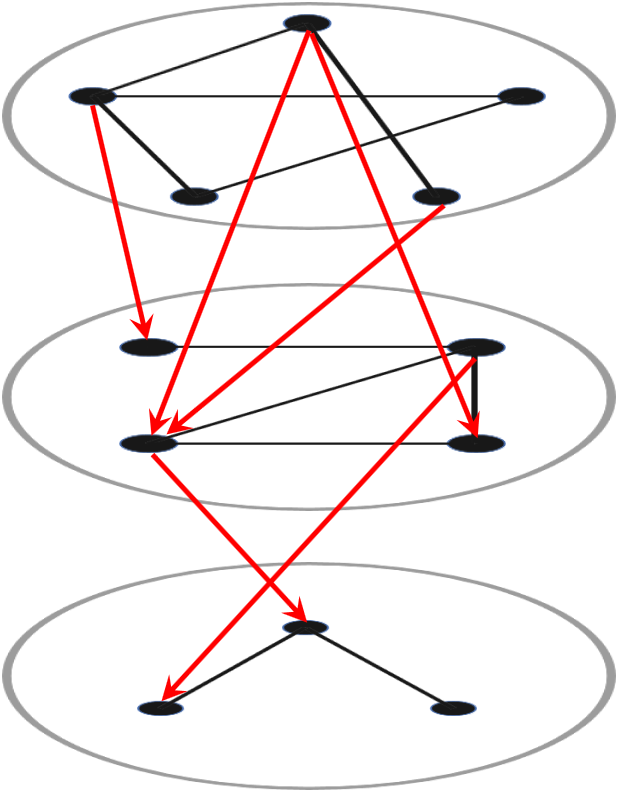
\includegraphics[height=.7\textheight]{formulation_5}
\end{minipage}

\end{frame}
%%%%%%%%%%%%%%%%%%%%%%%%%%%%%%%%%%%%%%%%%%%%%%%%%%%%%%%%%%%%%%%%

\begin{frame}
\frametitle{Multiple Multi-layered Gaussian Graphical models}

%
\begin{align*}
& \BE^k = (E_1^k, \ldots, E_q^k)^T \sim \cN_p (0, \Sigma_y^k); \quad
\Omega_y^k = (\Sigma_y^k)^{-1}\\
& \BY^k = \BX^k \bfB^k + \BE^k; \quad k = 1, 2, \ldots, K
\end{align*}
%

\begin{tabular}{ccc}
\hspace{1em} 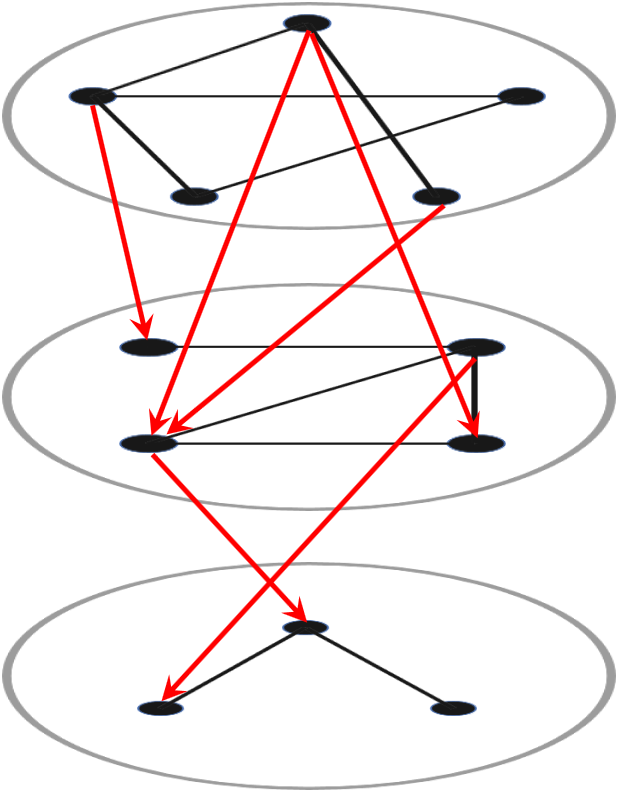
\includegraphics[width=.25\textwidth]{formulation_5} \hspace{1em} &
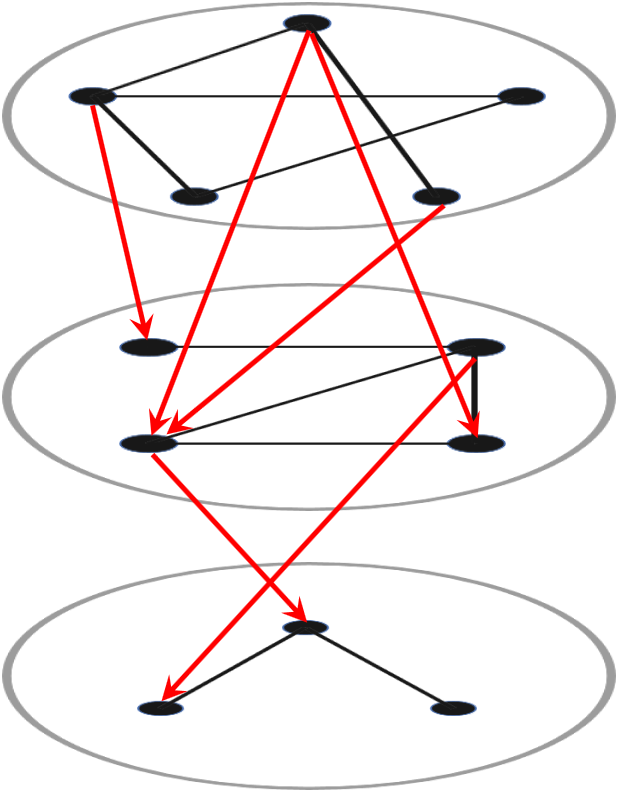
\includegraphics[width=.25\textwidth]{formulation_5} \hspace{1em} &
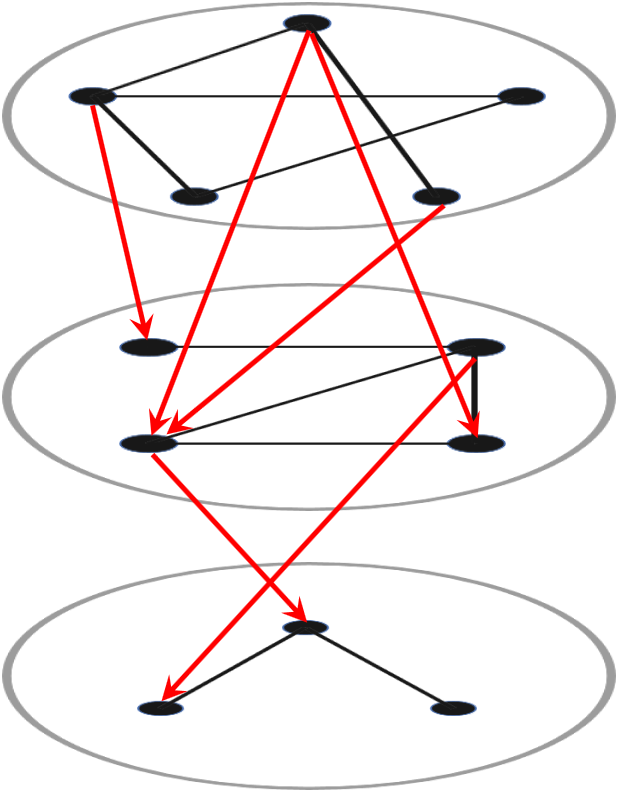
\includegraphics[width=.25\textwidth]{formulation_5} \hspace{1em} \\
$k=1$ & $k=2$ & $k=3$
\end{tabular}

\vspace{1em}
\begin{itemize}
\item We estimate $\{ \Omega_x^k, \Omega_y^k, \bfB^k \}$ jointly for all $k$ from a single model;

\item For $K=2$ and $i \in \{ 1, 2, \ldots, p\}$, we also provide a global test for $\bfb_i^1 = \bfb_i^2$, and do multiple testing for $b_{ij}^1 = b_{ij}^2, j = 1, 2, \ldots, q$.
\end{itemize}

\end{frame}
%%%%%%%%%%%%%%%%%%%%%%%%%%%%%%%%%%%%%%%%%%%%%%%%%%%%%%%%%%%%%%%%

\section{Model formulation, computation and theory}
%%%%%%%%%%%%%%%%%%%%%%%%%%%%%%%%%%%%%%%%%%%%%%%%%%%%%%%%%%%%%%%%

\begin{frame}
\frametitle{Preliminaries}

\begin{itemize}
\item $\cY = \{ \bfY^1, \ldots, \bfY^k\},
\cX = \{ \bfX^1, \ldots, \bfX^k\}, \cB = \{ \bfB^1, \ldots, \bfB^k \}$;

\item Group structures in X-network is denoted by
%
\[
\cG_x = \{\cG_{x,ii'}: i \neq i', 1 \leq i,i' \leq p \}
\]
%
Each $\cG_{x,ii'}$ is a partition of $\{ 1, \ldots, K\}$ denoting grouping over $k$ for the $(i,i')^{\Th}$ elements of the $X$-precision matrices. For example, for $K=5$,
%
\[
\cG_{x,12} = \{ (1,2),(3),(4,5)\}; \quad
\cG_{x,13} = \{ (1),(2,3),(4,5)\}
\]
%
\item Define $\cG_y = \{\cG_{y,jj'}: j \neq j', 1 \leq j,j' \leq q \}
$ similarly.
\item Group structures in $\cB$ is denoted by $\cH$, with each $h \in \cH$ being a collection of 3-tuples $(h_i,h_j,h_k)$ so that $1 \leq h_i \leq p, 1 \leq h_j \leq q, 1 \leq h_k \leq K$.
\end{itemize}

\end{frame}

%%%%%%%%%%%%%%%%%%%%%%%%%%%%%%%%%%%%%%%%%%%%%%%%%%%%%%%%%%%%%%%%
\begin{frame}
\frametitle{Neighborhood selection}

\begin{itemize}
\item {\bf For single GGM}: Estimate neighboring edges for each node, then refit.
%
\begin{align*}
\hat \bfzeta_i &= \argmin_{\bfzeta_i} \left\{ \frac{1}{n} \| \bfX_i - \bfX_{-i} \bfzeta_i \|^2 + \nu_n \sum_{i' \neq i} |\zeta_{ii'}| \right\};\\
\hat \Omega_x &= \argmin_{\Omega_x \in \cup_i \text{support} (\bfzeta_i)}
\{ \Tr (\bfS_x \Omega_x ) + \log \det(\Omega_x) \}
\end{align*}
%
Can do this because $\zeta_{ii'} = -\omega_{ii'}/\omega_{ii}$, so zeros of the precision matrix and neighborhood matrix are same.

\item {\bf For multiple GGM}: Incorporate penalty across different $k$ (JSEM: \cite{MaMichailidis15}).
%
\begin{align*}
\hat \bfzeta_i &= \argmin_{\zeta_i} \left\{ \sum_{k=1}^K \frac{1}{n_k} \| \bfX_i^k - \bfX_{-i}^k \bfzeta_i^k \|^2 + \nu_n \sum_{i' \neq i, g \in \cG_{x,ii'}} \| \bfzeta_{ii'}^{[g]} \| \right\};\\
\hat \Omega_x^k &= \argmin_{\Omega_x^k \in \cup_i \text{support} (\bfzeta_i^k)}
\left\{ \Tr (\bfS_x^k \Omega_x^k ) + \log \det (\Omega_x^k ) \right\}; \end{align*}
%
\end{itemize}
\end{frame}
%%%%%%%%%%%%%%%%%%%%%%%%%%%%%%%%%%%%%%%%%%%%%%%%%%%%%%%%%%%%%%%%

\begin{frame}
\frametitle{Our method}

\begin{center}
{\colrbf Joint Multiple Multi-Level Estimation (JMMLE)}
\end{center}

\vspace{1em}
We decompose the multi-layer problem into a series of two layer problems. For within-layer connections in the topmost layer, we use JSEM. For other connections we use JMMLE. 
%
\begin{figure}
\centering
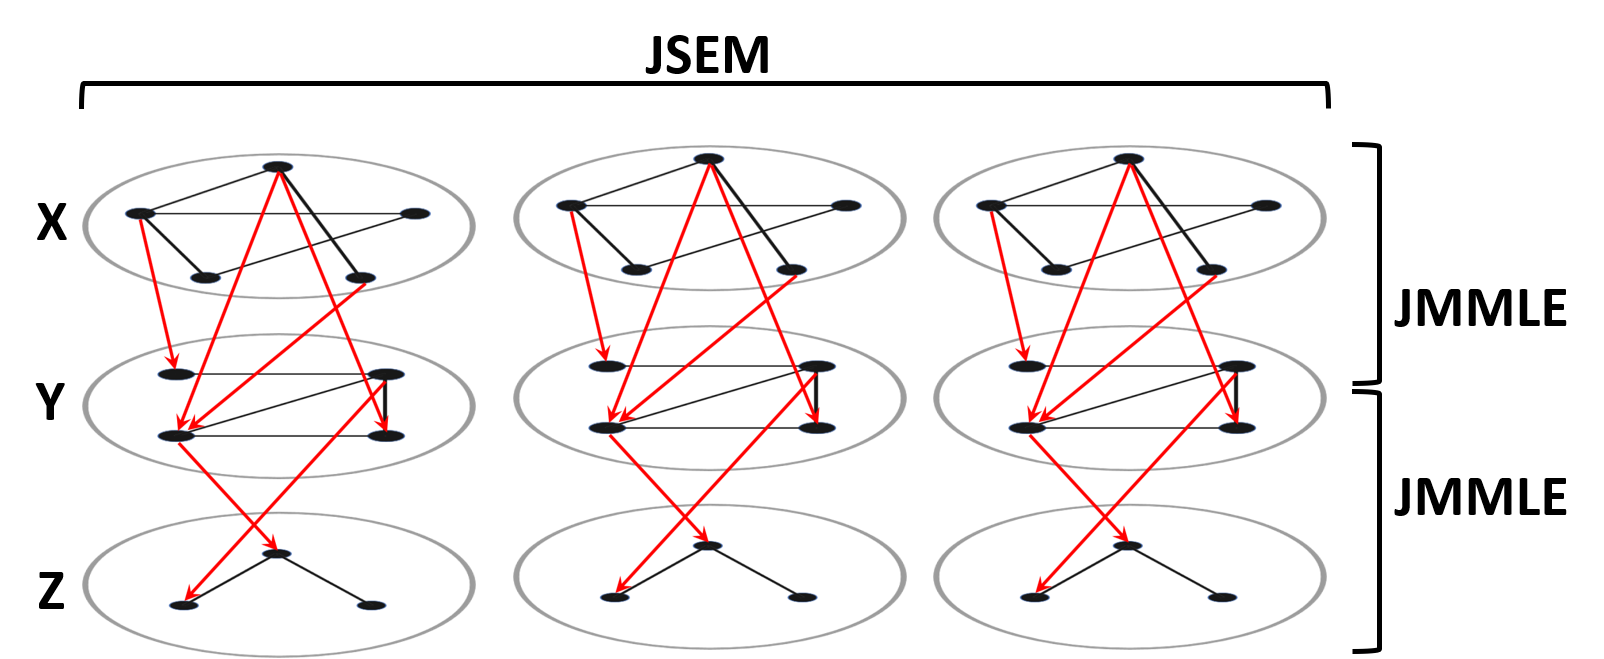
\includegraphics[width=.9\textwidth]{multilayer}
\end{figure}
\end{frame}

\begin{frame}
\frametitle{The JMMLE estimator}
We combine sparse neighborhood selection in the Y-network with sparse estimation of $\{ \bfB^k \}$.

Take $\Theta_j = (\bftheta_j^1, \ldots, \bftheta_j^K), \Theta = \{ \Theta_j \}_{j=1}^q$.

\begin{align*}
\{ \hat \cB, \hat \Theta \} &=
\argmin_{\cB, \Theta} \left\{ \sum_{k=1}^K \frac{1}{n_k} \sum_{j=1}^q
\left\| \bfY_j^k - ( \bfY_{-j}^k - \bfX^k \bfB_{-j}^k) \bftheta_j^k
- \bfX^k \bfB_j^k \right\|^2 \right.\\
& + \lambda_n \sum_{h \in \cH} \| \bfB^{[h]} \|
+ \gamma_n \left. \sum_{j' \neq j, g \in \cG_{jj'}} \| \bftheta_{jj'}^{[g]} \| \right\}\\
\hat \Omega_y^k &= \argmin_{\Omega_y^k \in \cup_i \text{support} (\bftheta_i^k)}
\left\{ \Tr (\bfS_y^k \Omega_y^k ) + \log \det (\Omega_y^k ) \right\}
\quad k = 1, 2, \ldots, K
\end{align*}
\end{frame}
%%%%%%%%%%%%%%%%%%%%%%%%%%%%%%%%%%%%%%%%%%%%%%%%%%%%%%%%%%%%%%%%
\begin{frame}
\frametitle{Computational algorithm}
\begin{align*}
\{ \hat \cB, \hat \Theta \} &= \argmin_{\cB, \Theta}
\left\{ f(\cY, \cX, \cB, \Theta) + P(\cB) + Q(\Theta) \right\}
\end{align*}

The objective function is biconvex, so we solve the above by the following alternating iterative algorithm:

\begin{enumerate}
\item Start with initial estimates of $\cB$ and $\Theta$, say $\cB^{(0)}, \Theta^{(0)}$.
\item Iterate:
%
\begin{align*}
\cB^{(t+1)} &= \argmin_\cB \left\{ f ( \cY, \cX, \cB, \Theta^{(t)}) + Q (\cB) \right\}\\
\Theta^{(t+1)} &= \argmin_\Theta \left\{ f ( \cY, \cX, \cB^{(t+1)}, \Theta) + P (\Theta) \right\}
\end{align*}
\item Continue till convergence.
\end{enumerate}
\end{frame}
%%%%%%%%%%%%%%%%%%%%%%%%%%%%%%%%%%%%%%%%%%%%%%%%%%%%%%%%%%%%%%%%

\begin{frame}
\frametitle{The two subproblems}
\begin{align*}
\hat \cB &=
\argmin_{\cB} \left\{
\sum_{k=K}^q \frac{1}{n_k} \sum_{j=1}^q
\left\| \bfY_j^k - ( \bfY_{-j}^k - \bfX^k \bfB_{-j}^k) \hat \bftheta_j^k
- \bfX^k \bfB_j^k \right\|^2
+ \lambda_n \sum_{h \in \cH} \| \bfB^{[h]} \| \right\}\\
&= \argmin_{\cB} \left\{ \sum_{k=1}^K \frac{1}{n_k}
\| (\bfY^k - \bfX^k \bfB^k) \bfT^k \|_F^2 +
+ \lambda_n \sum_{h \in \cH} \| \bfB^{[h]} \| \right\}
\end{align*}
%
where $t_{jj}^k = 1, t_{jj'}^k = - \theta_{jj'}^k$.

\begin{align*}
\hat \Theta &=
\argmin_{\Theta} \left\{ \sum_{k=K}^q \frac{1}{n_k} \sum_{j=1}^q
\left\| \bfY_j^k - ( \bfY_{-j}^k - \bfX^k \hat \bfB_{-j}^k) \bftheta_j^k
- \bfX^k \hat \bfB_j^k \right\|^2 
+ \gamma_n \sum_{j' \neq j, g \in \cG_{jj'}} \| \bftheta_{jj'}^{[g]} \| \right\}\\
&= \argmin_{\Theta} \left\{ 
\sum_{k=K}^q \frac{1}{n_k} \sum_{j=1}^q
\| \hat \bfE_j^k - \hat \bfE_{-j}^k \bftheta_j^k \|^2
+ \gamma_n \sum_{j' \neq j, g \in \cG_{jj'}} \| \bftheta_{jj'}^{[g]} \| \right\}
\end{align*}
%
where $\hat \bfE^k = \bfY^k - \bfX^k \hat \bfB^k$.

\end{frame}

%%%%%%%%%%%%%%%%%%%%%%%%%%%%%%%%%%%%%%%%%%%%%%%%%%%%%%%%%%%%%%%%

\begin{frame}
\frametitle{Non-asymptotic error bounds for $\hat \cB$}

For $\lambda_n \geq 4 \sqrt{| h_{\max} |} \BR_0 \sqrt{ \frac{ \log(pq)}{n}}$, the following hold with probability approaching 1 as $n \rightarrow \infty$,
%
\begin{align*}
\| \hat \bfbeta - \bfbeta_0 \|_1 & \leq \frac{48 \sqrt{ | h_{\max} |} s_\beta \lambda_n}{ \psi^*} \\
\| \hat \bfbeta - \bfbeta_0 \| & \leq \frac{12 \sqrt s_\beta \lambda_n}{ \psi^*} \\
\sum_{h \in \cH} \| \bfbeta^{[h]} - \bfbeta_0^{[h]} \| & \leq \frac{48 s_\beta \lambda_n}{ \psi^*}
\end{align*}
%
with $\psi^*, \BR_0$ being constants, and $\bfbeta = (\ve(\bfB^1)^T, \ldots, \ve(\bfB^K)^T)^T$, $| h_{\max} |$ the maximum group size in $\bfbeta_0$ and $s_\beta$ the sparsity of $\bfbeta_0$.
\end{frame}

%%%%%%%%%%%%%%%%%%%%%%%%%%%%%%%%%%%%%%%%%%%%%%%%%%%%%%%%%%%%%%%%
\begin{frame}
\frametitle{Error bounds for $\hat \Theta, \hat\Omega$}

For $\gamma_n = 4 \sqrt{| g_{\max}|} \BQ_0 \sqrt{ \frac{ \log(pq)}{n}}$, the following hold with probability approaching 1 as $n \rightarrow \infty$,
%
\begin{align*}
\| \hat \Theta_j - \Theta_{0,j} \|_F & \leq \frac{12 \sqrt{s_j} \gamma_n}{\psi} \\
\sum_{j \neq j', g \in \cG_y^{jj'}} \| \hat \bftheta_{jj'}^{[g]} - \bftheta_{0,jj'}^{[g]} \| & \leq \frac{48 s_j \gamma_n}{\psi} \\
\left| \text{support} (\hat \Theta_j) \right| & \leq
\frac{128 s_j}{ \psi}\\
\frac{1}{K} \sum_{k=1}^K \| \hat \Omega_y^k - \Omega_y^k \|_F & \leq
O \left( \frac{\sqrt S \gamma_n }{\sqrt K} \right)\\
\end{align*}
%
with $\psi, \BQ_0$ being constants, $| g_{\max} |$ the maximum group size in $\Theta_0$, $s_j$ the sparsity of $\Theta_j$ and $S = \sum_j s_j$.
\end{frame}

%%%%%%%%%%%%%%%%%%%%%%%%%%%%%%%%%%%%%%%%%%%%%%%%%%%%%%%%%%%%%%%%
\section{Hypothesis testing}
%%%%%%%%%%%%%%%%%%%%%%%%%%%%%%%%%%%%%%%%%%%%%%%%%%%%%%%%%%%%%%%%
\begin{frame}
\frametitle{Debiasing JMMLE estimates}

\begin{itemize}
\item Consider the case $K=2$, and suppose we are interested in testing if the effect of variable $i$ in the X-data is different across the two populations.
\vspace{1em}

\item For this we use the $i^{\text{th}}$ rows of the estimates $\hat \bfB^1$ and $\hat \bfB^2$.
\vspace{1em}

\item We debias these row vectors using the neighborhood coefficients in the X-network computed previously using JSEM:
%
In this setup, define the desparsified estimate of $\bfb_i^k$ as
%
\begin{align*}
\hat \bfc_i^k = \hat \bfb_i^k + \frac{1}{n t_i^k} \left( \bfX_i^k - \bfX_{-i}^k \hat \bfzeta_i^k \right)^T
(\bfY^k - \bfX^k \hat \bfB^k )
\end{align*}
%
for $k = 1,2$, where $t_i^k := ( \bfX_i^k - \bfX_{-i}^k \hat \bfzeta_i^k )^T \bfX_{-i}^k/n$.
\end{itemize}

\end{frame}
%%%%%%%%%%%%%%%%%%%%%%%%%%%%%%%%%%%%%%%%%%%%%%%%%%%%%%%%%%%%%%%%

\begin{frame}
\frametitle{Result}
Assume we have `good enough' estimators:
%
\[
\| \hat \bfzeta^k - \bfzeta_0^k \|_1 = O \left( \sqrt { \frac{\log p}{n}} \right); \quad
\| \hat \bfB^k - \bfB^k_0 \|_1 = O \left( \sqrt{\frac{\log (pq)}{n}} \right)
\]
\[
\left\| (\hat \Omega_y^k)^{1/2} - (\Omega_y^k)^{1/2} \right\|_\infty = O \left( \sqrt { \frac{\log q}{n}} \right)
\]
%
Also define
%
\[
\hat s_i^k := \sqrt{\| \bfX_i^k - \bfX_{-i}^k \hat \bfzeta_i^k \|^2/n}; \quad
m_i^k := \sqrt n t_i^k / \hat s_i^k
\]
%
Then for sample size satisfying $n \succsim \log (pq), \log p = o(n^{1/2}), \log q = o(n^{1/2})$ we have
%
\begin{align*}
\begin{bmatrix}
\hat \Omega_y^1 &\\
& \hat \Omega_y^2
\end{bmatrix}^{1/2}
%
\begin{bmatrix}
m_i^1 (\hat \bfc_i^1 - \bfb_i^1) &\\
&  m_i^2 (\hat \bfc_i^2 - \bfb_i^2)
\end{bmatrix}
\sim \cN_{2q} ({\bf 0}, \bfI) + o_P(1)
\end{align*}

\end{frame}
%%%%%%%%%%%%%%%%%%%%%%%%%%%%%%%%%%%%%%%%%%%%%%%%%%%%%%%%%%%%%%%%

\begin{frame}
\frametitle{Global test for $H_0: \bfb_{0 i}^1 = \bfb_{0 i}^2$ at level $\alpha, 0< \alpha< 1$}
\begin{enumerate}
\item Obtain the debiased estimators $\hat \bfc_i^1, \hat \bfc_i^2$;

\item Calculate the test statistic
%
$$
D_i = \left\| m_i^1 (\hat \Omega_y^1)^{1/2} \hat \bfc_i^1 - 
 m_i^2 (\hat \Omega_y^2)^{1/2} \hat \bfc_i^2 \right\|^2
$$
%

\item Reject $H_0$ if $D_i \geq \chi^2_{2q, 1-\alpha}$.
\end{enumerate}
\end{frame}
%%%%%%%%%%%%%%%%%%%%%%%%%%%%%%%%%%%%%%%%%%%%%%%%%%%%%%%%%%%%%%%%

\begin{frame}
\frametitle{Simultaneous tests for $H_0^{j}: b_{0 ij}^1 = b_{0 ij}^2$ at level $\alpha, 0< \alpha< 1$}

\begin{enumerate}
\item Calculate the pairwise test statistics $d_{ij}$ for $j = 1, \ldots, q$:
%
\[
d_{ij} = \frac{\tau_{ij}^1 \hat \bfc_{ij}^1 - \tau_{ij}^2 \hat \bfc_{ij}^2}{1/m_i^1 + 1/m_i^2}
\]
%
where $\tau_{ij}^k$ is the $(i,j)^{\Th}$ element of $(\hat \Omega_y^k)^{1/2}, k=1,2$.

\item Obtain the threshold
%
$$
\hat \tau = \inf \left\{\tau \in \BR: 1 - \Phi(\tau) \leq \frac{\alpha}{2 q}
\max \left( \sum_{j \in \cI_q} \BI( |d_{ij}| \geq \tau), 1 \right) \right\}
$$
%

\item For $j \in \cI_q$, reject $H_0^{j}$ if $|d_{ij}| \geq \hat \tau$.
\end{enumerate} 

\end{frame}
%%%%%%%%%%%%%%%%%%%%%%%%%%%%%%%%%%%%%%%%%%%%%%%%%%%%%%%%%%%%%%%%
\section{Simulation studies}
%%%%%%%%%%%%%%%%%%%%%%%%%%%%%%%%%%%%%%%%%%%%%%%%%%%%%%%%%%%%%%%%

\begin{frame}
\frametitle{Simulation setup}
\begin{itemize}
\item Number of categories ($K$) = 5;

\item Structured $\{ \Omega_x\}, \{\Omega_y\}, \cB$;

\item Groups in $\cB,\Omega_x$ are non-zero with probability $5/p$, and their elements come from Unif$(-1, -0.5) \cup (0.5,1)$;

\item Groups in $\Omega_y$ are non-zero with probability $5/q$, and their elements come from Unif$(-1, -0.5) \cup (0.5,1)$;

\item We generate size-$n$ i.i.d. samples $\bfX^k$ from $\cN_p(0, \Sigma_x^k)$, and $\bfE^k$ from $\cN_p(0, \Sigma_y^k)$, then obtain $\bfY^k = \bfX^k \bfB^k + \bfE^k$;
\item 100 Replications.

\end{itemize}
\end{frame}
%%%%%%%%%%%%%%%%%%%%%%%%%%%%%%%%%%%%%%%%%%%%%%%%%%%%%%%%%%%%%%%%

\begin{frame}
\frametitle{Evaluation metrics}
\begin{enumerate}
\item True positives-
%
\[
\text{TP} (\hat \cB) = \frac{\sum_k | \supp(\hat \bfB^k) \cup \supp (\bfB_0^k)|}{\sum_k | \supp (\bfB_0^k)| }
\]
\item True negatives-
%
\[
\text{TN} (\hat \cB) = \frac{\sum_k | \supp^c(\hat \bfB^k) \cup \supp^c (\bfB_0^k)|}{\sum_k | \supp^c (\bfB_0^k)| }
\]
%
\item Relative error in Frobenius norm-
%
\[
\text{rel.Frob} (\hat \cB) = \sum_{k=1}^K \frac{\| \hat \bfB^k - \bfB_0^k \|_F}{\| \bfB_0^k \|_F}
\]
%
\end{enumerate}

Same metrics are used for $\hat \Theta$.
\end{frame}
%%%%%%%%%%%%%%%%%%%%%%%%%%%%%%%%%%%%%%%%%%%%%%%%%%%%%%%%%%%%%%%%
\begin{frame}
\frametitle{Results}

\begin{scriptsize}
\begin{table}
    \begin{tabular}{c|ccc|ccc}
    \hline
    \multicolumn{7}{c}{{\bf Setting 1: $n=100, p=60, q=30, K=5$}}\\\hline
    Method        & TP($\hat\cB$)         & TN($\hat\cB$)         & rel.Frob($\hat\cB$) & TP($\hat\Theta$)   & TN($\hat\Theta$)   & rel.Frob($\hat\Theta$) \\\hline
    Joint (JMMLE) & 0.999 (2e-3) & 0.99 (0.01)   & 0.19 (0.02)  & 0.66 (0.06) & 0.95 (0.01) & 0.33 (0.02)      \\
    Separate      & 0.95 (0.02)   & 0.99  (2e-3) & 0.27 (0.03)  & 0.89 (0.02) & 0.63 (0.01) & 0.77 (0.04)      \\\hline
    \multicolumn{7}{c}{{\bf Setting 2: $n=100, p=30, q=60, K=5$}}\\\hline
    Method        & TP($\hat\cB$)         & TN($\hat\cB$)         & rel.Frob($\hat\cB$) & TP($\hat\Theta$)   & TN($\hat\Theta$)   & rel.Frob($\hat\Theta$) \\\hline
    Joint (JMMLE) & 0.996 (4e-3) & 0.99 (6e-3)   & 0.21 (0.01)  & 0.58 (0.04) & 0.98 (3e-3) & 0.32 (8e-3)      \\
    Separate      & 0.66 (0.04)  & 0.994  (1e-3) & 0.59 (0.03)  & 0.62 (0.03) & 0.81 (7e-3) & 0.43 (0.01)      \\\hline
    \multicolumn{7}{c}{{\bf Setting 3: $n=150, p=200, q=200, K=5$}}\\\hline
    Method        & TP($\hat\cB$)         & TN($\hat\cB$)         & rel.Frob($\hat\cB$) & TP($\hat\Theta$)   & TN($\hat\Theta$)   & rel.Frob($\hat\Theta$) \\\hline
    Joint (JMMLE) & 1.00 (0) & 1.00 (0)   & 0.12 (5e-3)  & 0.39 (0.04) & 0.996 (2e-3) & 0.30 (7e-3)      \\
    Separate      & 0.42 (0.03)   & 0.99  (1e-3) & 0.48 (0.02)  & 0.41 (0.02) & 0.73 (0.01) & 0.44 (0.02)      \\\hline
    \end{tabular}
\end{table}
\end{scriptsize}
\end{frame}
%%%%%%%%%%%%%%%%%%%%%%%%%%%%%%%%%%%%%%%%%%%%%%%%%%%%%%%%%%%%%%%%

\begin{frame}
\frametitle{Future work}

\begin{itemize}
\item Larger simulation: effect of signal strength and sparsity;
\vspace{1em}

\item Real data application, application to personalized medicine;
\vspace{1em}

\item Mediation analysis.
\end{itemize}
\end{frame}

\begin{frame}
\frametitle{References}
{\scriptsize
\bibliographystyle{plainnat}
\bibliography{IISAbib}
}
\end{frame}
%%%%%%%%%%%%%%%%%%%%%%%%%%%%%%%%%%%%%%%%%%%%%%%%%%%%%%%%%%%%%%%%


\begin{frame}
\centering
{\huge\textcolor{UniBlue}{\textbf{THANK YOU!}}}\\

\vspace{2em}

\vspace{1em}
{\colubf Questions?}
\end{frame}

\end{document}